\documentclass[8pt]{article}
\usepackage[breaklinks=true]{hyperref}
\usepackage[margin=0.5in]{geometry}
\usepackage[font=scriptsize,labelfont=bf,textfont={it}]{caption}
\usepackage{color}
\usepackage{graphicx}

\definecolor{pblue}{rgb}{0.13,0.13,1}
\definecolor{pgreen}{rgb}{0,0.5,0}
\definecolor{pred}{rgb}{0.9,0,0}
\definecolor{pgrey}{rgb}{0.46,0.45,0.48}

\usepackage{listings}
\lstset{language=bash,
  showspaces=false,
  showtabs=false,
  breaklines=true,
  showstringspaces=false,
  breakatwhitespace=true,
  commentstyle=\color{pgreen},
  keywordstyle=\color{pblue},
  stringstyle=\color{pred},
  basicstyle=\ttfamily,
  frame=single,
  moredelim=[il][\textcolor{pgrey}]{$$},
  moredelim=[is][\textcolor{pgrey}]{\%\%}{\%\%}
}

\lstdefinestyle{term}{language=bash,
  columns=fullflexible,
  showspaces=false,
  showtabs=false,
  breaklines=true,
  showstringspaces=false,
  tabsize=2,
  breakatwhitespace=true,
  commentstyle=\color{pgreen},
  keywordstyle=\color{pblue},
  stringstyle=\color{pred},
  basicstyle=\small\ttfamily,
  frame=single,
  moredelim=[il][\textcolor{pgrey}]{$$},
  moredelim=[is][\textcolor{pgrey}]{\%\%}{\%\%},
  upquote=true
}
\lstdefinestyle{sh}{language=bash,
  columns=fullflexible,
  showspaces=false,
  showtabs=false,
  breaklines=true,
  showstringspaces=false,
  tabsize=2,
  breakatwhitespace=true,
  commentstyle=\color{pgreen},
  keywordstyle=\color{pblue},
  stringstyle=\color{pred},
  numbers=left,
  stepnumber=1,
  basicstyle=\small\ttfamily,
  frame=single,
  moredelim=[il][\textcolor{pgrey}]{$$},
  moredelim=[is][\textcolor{pgrey}]{\%\%}{\%\%},
  upquote=true
}

\lstdefinestyle{py}{language=python,
  columns=fullflexible,
  showspaces=false,
  showtabs=false,
  breaklines=true,
  showstringspaces=false,
  tabsize=2,
  breakatwhitespace=true,
  commentstyle=\color{pgreen},
  keywordstyle=\color{pblue},
  stringstyle=\color{pred},
  numbers=left,
  stepnumber=1,
  basicstyle=\small\ttfamily,
  frame=single,
  moredelim=[il][\textcolor{pgrey}]{$$},
  moredelim=[is][\textcolor{pgrey}]{\%\%}{\%\%},
  upquote=true
}

\lstdefinestyle{txt}{
  columns=fullflexible,
  showspaces=false,
  showtabs=false,
  breaklines=true,
  showstringspaces=false,
  tabsize=2,
  breakatwhitespace=true,
  numbers=left,
  stepnumber=1,
  basicstyle=\small\ttfamily,
  frame=single,
  moredelim=[il][\textcolor{pgrey}]{$$},
  moredelim=[is][\textcolor{pgrey}]{\%\%}{\%\%},
  upquote=true
}


\title{\textbf{Week 06} \\
\Large Signals, C Programs, SetUID, SetGID, and Fun Stuff }
\author{
	Melvyn Ian Drag
}
\date{\today}


\begin{document}
\maketitle

\begin{abstract}
We'll learn about signal handling, C Programs, ssh, setuid, setgid, and talk about the exam.
\end{abstract}

\section{Machine Configuration 7:00 - 7:15}
For this lecture we will be using a \textbf{Debian 10 Digital Ocean server}.
Make sure you have one. Also, when you start the server, run the following
commands to make sure you can complete the exercises in this document.

\begin{lstlisting}[style=term]
root@machine$ apt update
root@machine$ apt install python3-dev vim git
# if prompted, say yes to everything.
root@machine$ git clone https://github.com/melvyniandrag/LinuxClassRepo.git
# now you have all the class stuff
\end{lstlisting}

{\Large Hurry and do this now! Don't ask me how to install python3 a half hour
from now. Don't ask how to clone the class repo at 8PM! It is important that you
keep up as we have alot to cover today!}

\section{Intro 7:15 - 7:20}

\textit{Start a podcast on Android phone, have someone call me during while the
podcast is playing and show that Android stops the podcast and starts the phone
call. When we hang up what happens? Either the podcast will start again or it
will not, this depends on how the phone is programmed.}

In \*nix a common thing you do is send signals to processes. You will sometimes
want to send information to a running program to make it do things. To get an
idea of what a signal is, imagine you are watching a youtube video on your
cell phone. If a phone call comes in, the video will pause, the phone app will
be opened, and you will be prompted to accept the call ( Other phones may
handle the situation differently, this is just a simple example ). How does your
phone ( which is a computer ) do this? I don't know, but in general when you
want to communicate with a running program you use signals. Maybe Android uses
signals when it makes programs communicate, maybe it doesn't.

 Signals are one important way we do \textbf{Interprocess Communication ( IPC )} on
Linux/BSD/Unix. The most common signals you'll want to send as an everyday Linux
user are \textbf{SIGINT} and \textbf{SIGTSTP}

\section{7:20 - 7:35 SIGTSTP and SIGINT}

\textit{The programs used throughout this lecture are in the Week06 Lecture directory in
the class repository that we  cloned at the beginning of class. }

\subsection{SIGINT}
We'll see what these do by running a small python program. Create this program
and run it on your computer ( note you don't need to create this program if you
have the class repo - it's there in the week 06 lecture directory ):

\lstinputlisting[language=Python]{runForever.py}

You run the program by typing:

\begin{lstlisting}[style=term]
root@machine$ python3 runForever.py
# the prompt will become unresponsive as the python program runs.
\end{lstlisting}

This program will run forever and hog up our terminal. How do we make it stop? We can send the \textbf{SIGINT} signal by typing "CTRL+C". Note that it stops. 

That may have been your first Python program. If you want to do the same thing
with bash, try running this program and seeing that it is ended with CTRL+C:

\lstinputlisting[language=bash,caption={runForever.sh}]{runforever.sh}

You have to ways to run this program:

\begin{lstlisting}[style=term]
user@machine$ bash runforever.sh
# interesting output
# end it by typing CTRL+C
\end{lstlisting}

Or you can use the "executable" permission I showed last week. There are two
examples of me making scripts executable in figure ~\ref{fig:executable}:

\begin{lstlisting}[style=term]
user@machine$ chmod +x runforever.sh
user@machine$ ./runforever.sh
# interesting output
# end it by sending the SIGINT signal with CTRL+C
# Do you see the emojis?
\end{lstlisting}

{\Large Question for class: do you remember another way to make the script
executable? How to do it with numbers? e.g. chmod 700 or chmod 777 or chmod 500,
etc.}

\begin{figure}[ht]
	\centering
	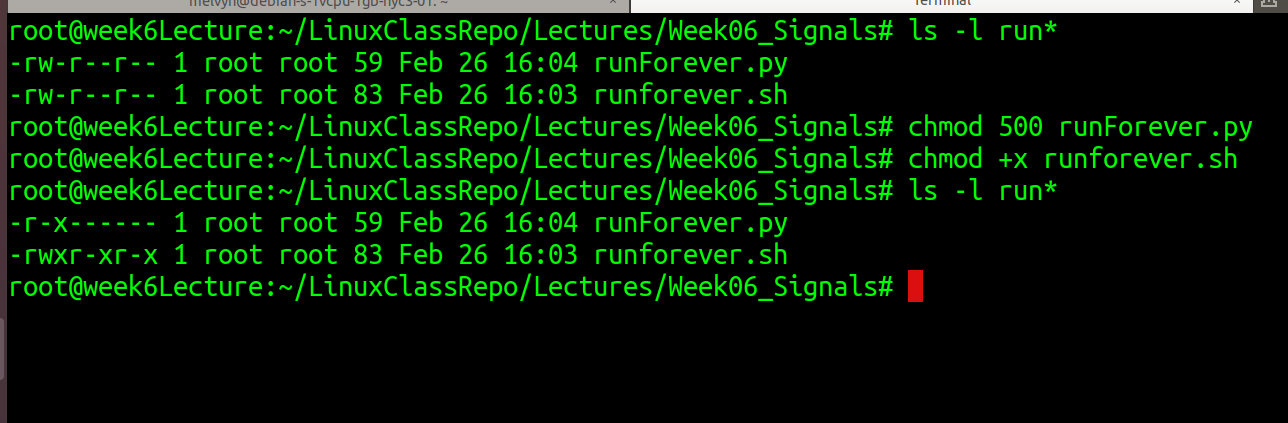
\includegraphics[width=0.7\textwidth]{Images/madeExecutable.png}
	\caption{Look how I make Python3 and Bash scripts executable! Since the have
the `shebang' line as the first line in the script I can run the scripts by
saying ./scriptname.sh or ./scriptname.py instead of saying python scriptname.py
or bash scriptname.sh}
	\label{fig:executable}
\end{figure}

\subsection{SIGTSTP}
Another thing you might want to do is just pause the program for a bit. We saw
sometihng like this with Android already - if you receive a phone call, the
podcast application is paused, not closed. In Linux you pause a program by sending it 
a \textbf{SIGTSTP}. This is done by typing CTRL+Z. To restart the program that you
 paused you can send it a \textbf{SIGCONT} command. To send a \textbf{SIGCONT}
 command is a little different. There is no keyboard shortcut like CTRL+XYZ to
send the SIGCONT signal. You must type:

\begin{lstlisting}[style=term]
user@machine$ kill -18 $PYTHON_PID # where $PYTHON_PID is the PID of the process you stopped.
\end{lstlisting}

To verify this works, run the python program, but this time stop and restart it
in the following way:

\begin{lstlisting}[style=term]
user@machine$ python3 runForever.py
# running 
# then type CTRL+Z
# should say the process was stopped.
user@machine$ pidof python3
1123 1345 7899 9999
# a list of numbers comes out - these are all the python processes on your
# computer. We want to restart the newest one, the one that you just stopped.
# The smaller numbers are programs that Linux is running for some reason or
# other.
# Dont worry about those. In this example, the stopped process id ( pid
# ) is 9999. 
user@machine$ jobs
[1] Stopped        python3 runForever.py
user@machine$ kill -18 9999
user@machine$ jobs
[1] Running python3 runForever.py &
# but the program is running in the background. To bring it to the foreground we
# use the fg command.
user@machine$ fg 1
# you will see the python process come to life.
# Do this a few more times until bored. Then type CTRL+C to kill the process
# with SIGINT once and for all.
\end{lstlisting}

\subsection{Verify the signals}
See figure ~\ref{fig:pythonsignals} for a screenshot of me running these
commands.

\begin{enumerate}
\item type \textit{pidof python} ( or \textit{python3} )
\item Run \textit{runForever.py}
\item Send \textbf{SIGINT} with the keyboard
\item type \textit{pidof python} ( or \textit{python3} )
\item There should be no pid there corresponding to your process.
\item Run \textit{runForever.py}
\item Send \textbf{SIGTSTP} with the keyboard
\item type \textit{pidof python} ( or \textit{python3} )
\item There \textbf{should} be a pid corresponding to your process.
\item Restart the process with \textit{kill -18 \$ PID}
\item Type \textit{jobs}
\item Type \textit{fg \$JOB\_ID}
\item Kill the process so it doesn't hog memory.
\end{enumerate}

\begin{figure}[ht]
	\centering
	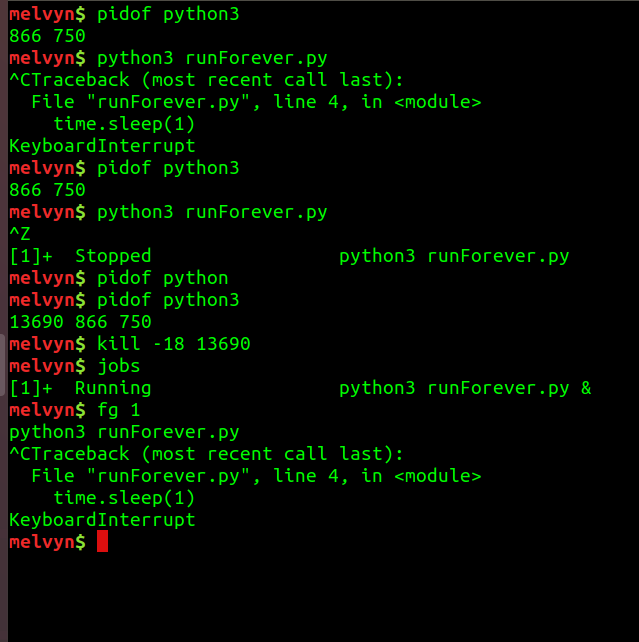
\includegraphics[width=0.7\textwidth]{signals.png}
	\caption{Look at home I send to python3}
	\label{fig:pythonsignals}
\end{figure}

\section{7:45-7:55 jobs vs processes}
Note I used the \textit{jobs} command above. That command lists the processes started by the current shell. If you start a new shell and type \textit{jobs} there will be no output, because your new shell didn't do anything yet.
There are two similar things happening here. The commands I've been using a bit
are \textit{pidof} and \textit{jobs}, and they both seem to report back some
number corresponding to a running program. All running programs are processes,
and they all get a system-wide \textit{pid} ( as always I'm not 100\% sure what
that stands for. \textit{process identifier} ? Or maybe \textit{process
identification} ? Whatever, pid is good enough). Every program that has been
started in the current bash session gets a job id tied to it. This job id will
not be visible to other bash sessions. The pid will be visible to everyone,
however.

Remember:
\begin{itemize}
\item all running programs are called processes and have a pid
\item all running programs are called processes and have a pid
\item all running programs are called processes and have a pid
\item all running programs are called processes and have a pid
\end{itemize}

never forget:

\begin{itemize}
\item all programs started by my shell are called jobs and have a job id.
\item all programs started by my shell are called jobs and have a job id.
\item all programs started by my shell are called jobs and have a job id.
\item all programs started by my shell are called jobs and have a job id.
\end{itemize}

To emphasize what I've said before, look how I start a job in one shell, then
start another shell and the job is not listed! See figure ~\ref{fig:jobs}

\begin{figure}[ht]
	\centering
	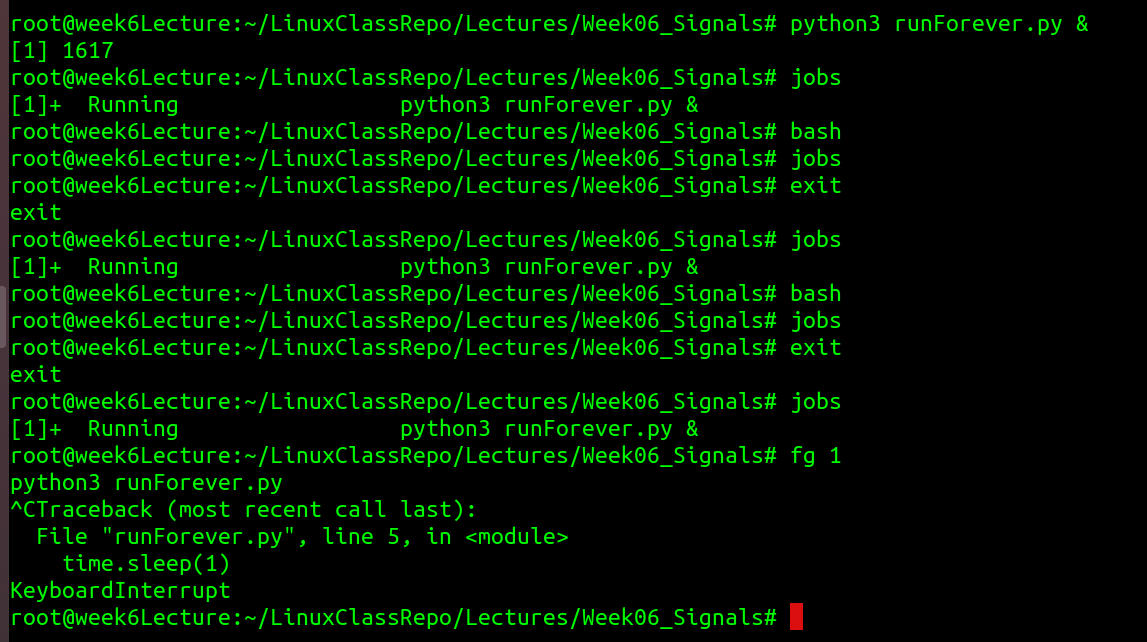
\includegraphics[width=0.7\textwidth]{Images/jobsAndBashShells.png}
	\caption{Start a background process with \&. List jobs and see its there.
start new bash shell. Type jobs. The job is gone! It's only property of the
parent shell, not the subshell. See when I type exit, the job is listed! Do this
a few times til it makes sense. Kill the process by foregrounding it, then
sending ctrl+c.}
	\label{fig:jobs}
\end{figure}


\section{{\color{red} 7:55-8:10 Exercise + break: ssh practice}}

I've given you alot of information. To practice what we learned last week, I
want you ssh into a classmate's digital ocean server. Here's how:

\begin{enumerate}
\item Fork one of your classmate's github repos
\item add your ssh public key to the repo
\item make a pull request
\item your classmate must merge the pull request on github
\item your classmate must create a user for you on his or her machine
\item your classmate must add your ssh public key to the file:
/home/YOURUSERNAME/.ssh/authorized\_keys
\item your classmate must run `service sshd restart' ( either as root or as a
sudoer )
\item you must try to ssh in like : ssh yourusername@machineipaddress
\end{enumerate}

\section{ kill }
You use the \textit{kill} command to send a signal to a process. Did you read
that last sentence? If you go on a job interview and the interviewer asks you:

\begin{verbatim}
Hello job candidate, do you know how to send a signal to a process on Linux?
\end{verbatim}

You had better know how to answer. I showed you one example wherein we sent an 18 to a process. You can see all of the signals available to send by typing 

\begin{lstlisting}
user@machine$ kill -l
\end{lstlisting}

You will see in the list are two of the signals I already showed you - the ones
I called `the most important signals'. Those are SIGINT and  SIGTSTP. Ask the
lass what the corresponding numbers are. These signals are known by the numbers
you just told me, SIGINT, INT, SIGTSTP and TSTP. The signal
18 is also known as SIGCONT or simply CONT. 
Using the kill command you can send these signals in three ways:

\begin{itemize}
\item Using the signal name e.g \textbf{CONT}
\item Using `SIG' + the signal name e.g. \textbf{SIGCONT}
\item Using the numeric code for the signal e.g. 18
\end{itemize}

In this lecture we're going to focus on the following signals:

\begin{enumerate}
\item SIGINT
\item SIGKILL
\item SIGTERM
\item SIGSTOP
\item SIGTSTP
\end{enumerate}

though there are more signals, this should be enough to get you started. And if you want to learn more you of course can go get a book. We're going to look at when you use each one of the above and how programs handle them when they are received. I think these are the most interesting of the 64 signals.

To know about the \textit{kill} command: \textit{kill} can take either pids or
job ids. So you can type either

\begin{lstlisting}[style=term]
user@machine$ jobs
[1] Stopped python3 program.py
user@machine$ kill -SIGINT %1
# program.py terminated
\end{lstlisting}

or you can type

\begin{lstlisting}[style=term]
user@machine$ pidof python3
100 145 1982
user@machine$ kill -SIGINT 1982
# python3 program terminated.
\end{lstlisting}

Without further ado, let's test the signals

\begin{lstlisting}
user@machine$ python3 runForever.py & # ampersand puts it in the background
user@machine$ jobs
[1]+Running   python3 runForever.py &
user@machine$ kill -20 %1 # or kill -20 $PIDOF_PYTHON. kill takes job ids or pids
user@machine$ jobs
#stopped
user@machine$ kill -18 %1
user@machine$ jobs
# it's running again
user@machine$ fg 1
user@machine$ [type ctrl + z]
\end{lstlisting}

We just sent \textbf{SIGCONT} and \textbf{SIGTSTP} using the numeric codes for them. Remember that we got the numeric codes by looking at the output of \textit{kill -l}. You'll note that, while the command is called \textit{kill}, it does more than kill. It can send all kinds of signals.

There is a signal related to \textbf{SIGTSTP} called \textbf{SIGSTOP}.
The difference between them is that \textbf{STOP} cannot be ignored and typically comes from a program. \textbf{TSTP} can be ignored. Depending on how much you've used linux, you may or may  not have been in a situation where you were mashing \textit{CTRL+C} over and over again, but the program wouldn't stop! By the end of tonight we'll write some code showing how that happens. Just know, that by the design of the Linux OS, \textbf{STOP} signals cannot be ignored.

\begin{lstlisting}
user@machine$ python runForever.py &
user@machine$ jobs
[1]+ Running python runForever.py &
user@machine$ kill -STOP %1
user@machine$ jobs
# it's stopped
user@machine$ kill -18 %1
user@machine$ jobs 
# it's running
user@machine$ fg 1
user@machine$ [type ctrl + z]
\end{lstlisting}

\section{An example of a pesky program}
{\Large no time now. if class ends early tell students to remind me and I'll
show them an example of a program that ignores signals.}

Before I told you that there are programs that just won't stop. Even though you
say SIGINT, the program will ignore you. Here is an example of such a program. I
use a tool called pdflatex to compile the \LaTeX source code for these lecture
notes into pretty pdfs for you. The \LaTeX compiler will refuse to respond the
the CTRL+C command when you try to make it stop.

TODO show students how to install pdflatex, get them a little sample .tex file
to compile, and show them how the compiler, when it encounters a bug in the
source code, will not exit even if you say CTRL+C.


\section{fg and bg}
You'll note I've used \textit{fg} a bit. This command takes a job id and puts it in the foreground. When you continue a job with \textbf{SIGCONT} it starts in the background. You have to bring it back into the foreground with \textit{fg} so you can interact with it e.g. send it a \textbf{SIGINT}. \textit{bg} has the opposite effect of putting a job in the background, like we did with \textit{\&}

\section{INT, TERM, KILL; Understanding Ignorable Signals}
\textbf{INT} is sent when you hit `CTRL+Z` on your keyboard. It interupt the
process and makes it stop. `SIGINT` can also be sent will \textit{kill}.
\textbf{SIGTERM} and \textbf{SIGINT} are approximately the same thing,
differences in their behavior are left up to the application developer. I'll
show you more about this later when we write some little C programs that will
ignore signals. You should now send \textbf{INT} and \textbf{TERM} to the \textit{runForever} program and you will see that both end the process. \textbf{KILL} is like \textbf{INT} or \textbf{TERM} but it cannot be ignored.

The number for KILL aka SIGKILL is 9. Remember, this signal cannot be blocked or
ignored. You can always send signal -9, no matter what is happening this signal
will work. It cannot be blocked or ignored! In any Linux system administration
book you read you will see thei \textbf{warning: `NEVER USE -9!`}. We have just
seen that processes can deliberately ignore or block signals if interruption
would cause some serious system harm. But sometimes, we just want the darned
process to stop! You can use SIGKILL under very dire circumstamstances, because
issuing this signal could cause file corruption!

Actually, thats what they say. I use \textbf{SIGKILL} sometimes and don't worry about it. My reason for doing so is boring to explain. I encourage you to read the following posts to develop your own opinion of whether or not to use SIGKILL/KILL/9

\begin{itemize}
\item \url{https://www.reddit.com/r/linux/comments/4b1mwh/do_not_use_sigkill/}
\item \url{https://unix.stackexchange.com/questions/281439/why-should-i-not-use-kill-9-sigkill}
\item \url{http://turnoff.us/geek/dont-sigkill/}
\item \url{https://unix.stackexchange.com/questions/8916/when-should-i-not-kill-9-a-process}
\end{itemize}

Whether you use the following code or not in your daily life, on your own laptop . . .

\begin{lstlisting}
user@machine$ kill -9 $pid
\end{lstlisting}

when you are in the office make sure you use \textbf{SIGINT} and \textbf{SIGTERM} first or your colleagues might look down on you as a reckless person.

\section{{\color{red} 8:30-8:40 EXERCISE: C Programming Warmup + A Break}}
{\color{green} Allow students to go to bathroom, talk amongst themselves for a
few minutes. The task during these few minutes is to get the helloworld.c file
using wget or whatever other means they want, then compile and run it as shown
below. After the break we'll move on to the signal handlers}.

We are going to write some C programs now. C is a language that is very intimately related to Linux. It looks and feels somewhat like other languages like 
\begin{enumerate}
\item Java
\item C\#
\item C++
\item But has many similarities to others. . .
\end{enumerate}

So if you have any experience with those languages, you'll more or less be able to read C.
Example program:

\lstinputlisting[language=C]{helloworld.c}

To compile and run this code you need to install the C compiler gcc, and then
compile and run the code.:

\begin{lstlisting}
user@machine$ sudo apt update
user@machine$ sudo apt install build-essential
user@machine$ gcc helloworld.c -o helloworld # compile the code
user@machine$ ./helloworld # run the code
\end{lstlisting}

\section{8:40 - 9:00 Writing Custom Signal Handlers With C}

We will change the behavior now. Run the code. From a separate terminal window, send kill signals. Then inspect the return code of the running process and see how we customized the return valu based on which signal we received. Remember that in our first assignment we looked at \$? to see how a program ended. You can return different values not just fro mbash scripts, as we've done with `return` and `exit` statements up until now. Your software can be programmed to return values too.

Returning to our discussion of signals, signals can be caught,  ignored, or blocked.

Most important thing for these three samples

{\LARGE GO SLOOOOOOOOW}

{\LARGE Open two Terminals and show how you send various signals to the process using \textit{kill}}

{\LARGE When appropriate ( i.e. TSTP or INT ) also show you can use CTRL+C and CTRL+Z}

\subsection{01\_signal\_handler.c}
This code shows the Linux programs can choose how to handle signals.

We will change write come code to change signal handling behavior now. Open `01*.c` on your computer and have a look at it. This is a small C program that registers two signal handlers. Remember, all these linux command line tools we are using like mv, cp, etc. are all simple C programs like the one we are writing now. They all register signal handlers like we are going to do now, and that's how the programs know what to do when you type CTRL+C or CTRL+Z on the keyboard, or what to do when you send a command with \textit{kill}

\begin{center}
\textbf{modify the program, compile, run. Allow students a few minutes to change the messages returned by SIGINT and SIGTERM. }
\end{center}

\lstinputlisting[language=C]{SignalHandlers/01_signal_handler.c}
\subsection{How to compile?}
Go to the SignalHandlers directory and type:

\begin{lstlisting}
user@machine$ gcc 01_signal_handler.c -o 01.out #compile
user@machine$ ./01.out #run
\end{lstlisting}

\subsection{02\_ignore.c}
This example shows that we can ignore a signal! We can tell a program to ignore a signal. 

What happens if you tell a program to ignore a signal that is unignorable?
\lstinputlisting[language=C]{SignalHandlers/02_ignore.c}

\subsection{03\_block.c}
This example shows that programs can temporarily refuse to handle signals. This is done with blocking. This program temporarily blocks a signal - can you see which one?

Try to send the signal while it is blocked and see what happens!!

\lstinputlisting[language=C]{SignalHandlers/03_block.c}

\section{Summary}

What can happen with signals?

\begin{itemize}
\item They can be handled
\item They can be ignored
\item They can be blocked
\end{itemize}

this is important, repeat it to yourself:

What can happen with signals?

\begin{itemize}
\item They can be handled
\item They can be ignored
\item They can be blocked
\end{itemize}

and once more for good measure:

What can happen with signals?

\begin{itemize}
\item They can be handled
\item They can be ignored
\item They can be blocked
\end{itemize}

\section{What are signals?}
Signals are a form of interprocess communication used in Linux. There are many interprocess communication mechanisms, this is just one of them. If you've never heard of IPC, just know it is all around you when you are using computers. For example, consider the case when you are on your telephone and you're listening to music. When a phone call comes in, the music is probably paused and the phone app is brought up on the screen. The operating system on your phone needed an IPC mechanism to detect that the phone process was in some active state and that other interfering processes need to take action while the call is active. Depending on how the software is written on your phone, the music might resume playing when you hang up, and the music app might come to the foreground on your screen. Or maybe it stays paused and you have to manually reopen the app and hit 'play' again. Or maybe something else happens.

IPC might also be used if you have two processes on a device - maybe you have one process listening for radio transmissions and another on that turns a motor. If the radio receiver receives a signal, maybe you want another process to turn a motor and open your garage door or something.

There are many ways to do IPC, even on Linux there are a bunch of IPC mechanisms. Signals is just one of them.

\section{9:00 - 9:05 Water break}
I'll probably be exhausted and need a break. Let's take 5 since the students
just got alot of information. Show the BSD and Mac if they want to check one
out.

\section{9:00 - 9:20 SetUID and SetGID}
\subsection{TL;DR}
In the next few minutes we're going to write a program that you can run as a
non-root user and  \textit{cat} a file belonging to root. This shouldn't happen!
Root's files should not be visible to a non root user. But it can if you know
this cool trick. 

\subsection{Introduction}
There are some special permissions that can be assigned to executables in Linux. You can trick your operating system into running a process as root, even though you are not root. The idea being, maybe you have a very trusted program that needs to do some root stuff. You are absolutely sure that the root stuff it does will not destroy your system, so you want to allow other users to do the root stuff even though they aren't root. <Flesh this out with some more discussion until it is clear>. 
  
Let's set up our machine for the next example. Login to digital ocean and create
a non-root user. Then, as root, create a file \textbf{/root/hello.txt}.

\begin{lstlisting}[style=term]
root@machine$ adduser calisto
# do the stuff
root@machine$ pwd
/root
root@machine$ vim hello.txt
# add some stuff to the file
root@machine$ cat hello.txt
this is roots file!
root@machine$ su - calisto
calisto@machine$ cat /root/hello.txt
cat: /root/hello.txt: Permission denied
\end{lstlisting}

So, as expected, `calisto' cannot peek inside root's files. Let's hack our
machine using the setuid bit to allow calisto to have a peek.

One quick thing - before we go any further let's make sure `calisto' is a
sudoer, we'll need that in a bit.

\begin{lstlisting}[style=term]
root@machine$ usermod -a -G sudo calisto
\end{lstlisting}

\subsection{uid}
In Linux, all users have a user id. You can get your user id from the command line by typing `id`. We haven't talked about this uid yet, and we certainly haven't used it, but it has been there all along. Today we will see what it is and we'll use it.

Try this:
\begin{lstlisting}
notRoot@machine$ id
# nonzero number
nonRoot@machine$ sudo su -
root@machine$ id
# see id is 0. Root's id is always 0.
\end{lstlisting}

So now we know what the uid of the root user is. Check out this program

\lstinputlisting[language=C]{setuid_setgid/execve_setuid.c}

There is alot to see in this code but the main idea is the following line:

\begin{lstlisting}[language=C]
char* const cat_argv[4] = { "/bin/sh", "-c", "cat /root/hello.txt"};
\end{lstlisting}

This code is trying to run the shell command \textit{cat /root/hello.txt} from a
nonroot user ( calisto in our case ). This is no good - as we've already seen,
only root can do that!

We see that with this program we make a few calls to getuid() and a few calls to setuid().
 You don't have to worry too much about this program - if you don't know C it
will the heck out of you. That's why I've chosen this simple and illustrative program.  
The main idea is that you see some source code here that calls these mysterious functions
getuid() and setuid()! We can change our user id while the program is running to trick the computer into thinking you are root!

`getuid` returns the user id of the user running the program.

We will first compile this normally and run it. You will see it fails and it exits with the value 1.

\begin{lstlisting}
calisto@machine$ gcc execve_setuid.c -o setuid
calisto@machine$ ./setuid
...
error msg
calisto@machine$ echo $?
1
\end{lstlisting}

This is because our program setuid exited with an error code ( nonzero ).

To make this work, we will have to change the ownership, the group, and the permissions.

\begin{lstlisting}
calisto@machine$ ls -l setuid # we need to change this stuff
-rwxr-xr-x 1 calisto calisto 17056 Feb 26 18:00 setuid
calisto@machine$ sudo chown root:root setuid
calisto@machine$ ls -l setuid # this changes the owner and group of the file
-rwxr-xr-x 1 root root 17056 Feb 26 18:00 setuid
calisto@machine$ sudo chmod +s setuid
calisto@machine$ ls -l setuid
-rwsr-xr-x 1 root root 17056 Feb 26 18:00 setuid
calisto@machine$ ./setuid
# it works!
\end{lstlisting}

So you see that both user and group have an `s` where there used to be an `x`. This means that the program can setuid() and setgid(). For this example we only wanted to setuid(), so we can just set u+s. 

\begin{lstlisting}
calisto@machine$ ls -l setuid # both user and group have 's'  i.e. rwsr-s....
-rwsr-sr-x 1 root root 17056 Feb 26 18:00 setuid
calisto@machine$ sudo chmod g-s setuid
calisto@machine$ ls -l setuid # now in the group permissions it is r-x
-rwsr-xr-x 1 root root 17056 Feb 26 18:00 setuid
calisto@machine$ ./setuid
# still works
\end{lstlisting}

Notice if we make group have `+s` but take the privilege away from user, 

\begin{lstlisting}
calist@machine$ sudo chmod u-s,g+s setuid
calisto@machine$ ls -l setuid
# you should understand the expected output now
calisto@machine$ ./setuid
# fails
\end{lstlisting}

Also, rememberwhen we were setting permissions using the octal notation? You can do that for this as well. There is no setAllID, there isonly setuid and setgid
So set uid is a 4, setgid is a 2, but what does the 1 correspond to? Not a big deal, I'll leave it here for you to read if you're curious! https://askubuntu.com/questions/432699/what-is-the-t-letter-in-the-output-of-ls-ld-tmp . So getting back to octal numbers and setuid/setgid we can set the permissions to r-sr-xr-x by saying `chmod 4555`. We can set the permissions to `r-xr-sr-x` with `chmod 2555`. Etc.

{\Large Do an example with the class setting the setuid/setgid bit using octal
notation!}

\section{9:20 - 9:45 Discussion of homework}
\subsection{Problem 1}
I just showed you a bit about setuid. Just recreate what I just showed you.

\subsection{Problem 2}
Look at the cool shell scripts book. I told you about signal handlers today.
Then I showed you how to do signal handling in C. Then I showed you how various
programs handle various signals. Now I want you to read a little article I found
online that explains how to handle signals in bash, and I want you to write some
code. The article may be gone from the internet. 

If you look here:

\url{linuxjournal.com} you'll see a notice that the company is dead, there
wasn't enough money to support the magazine. So the articles are on the internet
until they don't feel like paying for the webserver anymore. That could happen
at any moment. Very sad that they couldnt get enough money to stay afloat, the
magazine had many good articles. 

Anyway, the one you need to read is / was here:

\url{https://www.linuxjournal.com/article/10815} 

and in the event that it disappears it's in the Homework/Week06\_XX directory of
this repo.

You must read that article. 

For the homework I want you to make this state capital game work. Then I want
you to make it ignore the SIGINT command using the information you glean from
that article. As it is now, it does not ignore SIGINT( CTRL+C ). Look in figure
~\ref{fig:notIgnoring} and see that I stop the code by sending CTRL+C.

\begin{figure}[ht]
	\centering
	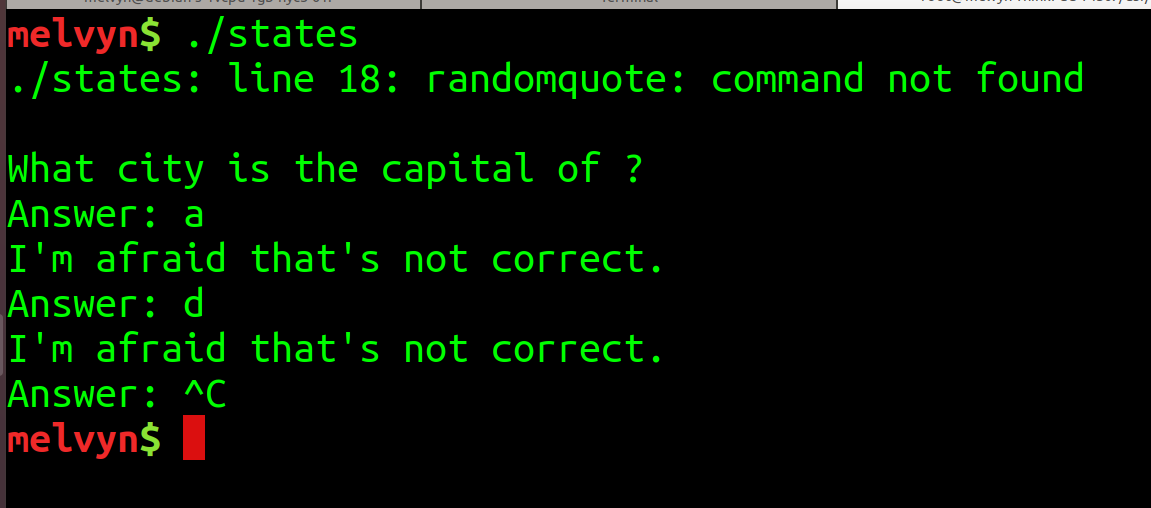
\includegraphics[width=0.7\textwidth]{Images/homework.png}
	\caption{The game isn't 100\% functional, I did the minimum to be able to
show you what I'm talking about. Notice that when I type CTRL+C, the game stops.
See the \^{}C on the screen? That means I typed CTRL+C.}
	\label{fig:notIgnoring}
\end{figure}

\subsection{Problem 3}
A little silly thing to do. 

\subsection{Discord}
I put a little server online for people to discuss things and share ideas and
reach out to me for help if you need it. Email is a crappy format for discussing
code in my opinion. discord lets you share nicely formatted code + images
easily, so it's better to just use that.

\end{document}
